%Dokumentklasse
\documentclass[a4paper,12pt]{scrreprt}
%\usepackage[left= 3.5cm,right = 2cm, bottom = 2 cm]{geometry}
\usepackage[left= 4.5cm,right = 1.5cm, bottom = 2.5 cm]{geometry}
\addtolength{\footskip}{-0.5cm}
\usepackage[onehalfspacing]{setspace}
% ============= Packages =============

% Dokumentinformationen
\usepackage[hyphens]{url}
\usepackage[
pdfsubject={},
pdfauthor={Ricardo Valente de Matos},
pdfkeywords={},	
%Links nicht einrahmen
hidelinks,
breaklinks=true
]{hyperref}
% Standard Packages
\usepackage[utf8]{inputenc}
\usepackage[ngerman]{babel}
\usepackage[T1]{fontenc}
\usepackage{graphicx, subfig}
\graphicspath{{img/}}
\usepackage{fancyhdr}
\usepackage{lmodern}
\usepackage{color}

\usepackage{dirtree}

\usepackage[style=ieee, sorting=nty, urldate =comp, backend=bibtex]{biblatex}
\addbibresource{Literatur.bib}

%\usepackage[numbers]{natbib}
%\bibpunct{(}{)}{;}{a}{,}{,}

\usepackage{listings}

% zusätzliche Schriftzeichen der American Mathematical Society
\usepackage{amsfonts}
\usepackage{amsmath}
\usepackage{float}

\usepackage{tabularx}
\usepackage{multirow}
\usepackage{enumitem}

%nicht einrücken nach Absatz
\setlength{\parindent}{0pt}
\RedeclareSectionCommand[beforeskip=0pt]{chapter}
\usepackage{listings}
\usepackage{color}
\definecolor{lightgray}{rgb}{.9,.9,.9}
\definecolor{darkgray}{rgb}{.4,.4,.4}
\definecolor{purple}{rgb}{0.65, 0.12, 0.82}

\lstdefinelanguage{JavaScript}{
	keywords={typeof, new, true, false, catch, function, return, null, catch, switch, var, if, in, while, do, else, case, break},
	keywordstyle=\color{blue}\bfseries,
	ndkeywords={class, export, boolean, throw, implements, import, this},
	ndkeywordstyle=\color{darkgray}\bfseries,
	identifierstyle=\color{black},
	sensitive=false,
	comment=[l]{//},
	morecomment=[s]{/*}{*/},
	commentstyle=\color{purple}\ttfamily,
	stringstyle=\color{red}\ttfamily,
	morestring=[b]',
	morestring=[b]"
}

\lstset{
	language=JavaScript,
	backgroundcolor=\color{lightgray},
	extendedchars=true,
	basicstyle=\footnotesize\ttfamily,
	showstringspaces=false,
	showspaces=false,
	numbers=left,
	numberstyle=\footnotesize,
	numbersep=9pt,
	tabsize=2,
	breaklines=true,
	showtabs=false,
	captionpos=b
}


% ============= Kopf- und Fußzeile =============
\pagestyle{fancy}
%
\lhead{}
\chead{}
\rhead{\slshape \leftmark}
%%
\lfoot{}
\cfoot{\thepage}
\rfoot{}
%%
\renewcommand{\headrulewidth}{0.4pt}
\renewcommand{\footrulewidth}{0pt}

% ============= Package Einstellungen & Sonstiges ============= 
%Besondere Trennungen
\hyphenation{De-zi-mal-tren-nung}

\newcommand{\hiddenchapter}[1]{
	\chapter*{{#1}}
}

%-------------

\newcommand{\todo}[1]{\textcolor{red}{ToDo:} #1\marginpar{<--hier}}

% ============= Dokumentbeginn =============

\begin{document}
%Seiten ohne Kopf- und Fußzeile sowie Seitenzahl
\pagestyle{empty}

\begin{center}
	\begin{tabular}{p{\textwidth}}
		
		\begin{center}
			\textbf{\Large{Thesis zur Erlangung des akademischen Grades Bachelor of Science (B. Sc.)}}
		\end{center} \\ \\
		
		\begin{center}
			\LARGE{\textsc{
					%\textit{\emph{adesso Staffing Advisor Lab}}\\
					%Konzeption und prototypische Entwicklung der Struktur und Architektur einer Softwareplattform für Transparenz in KI-Anwendungen
					Automatisierung der Informationsgewinnung in Bedarfsmeldungen
			}}
		\end{center}
		
		\\
		
		
		
		\begin{center}
			von
		\end{center}
		
		\begin{center}
			\large{\textbf{Ricardo Valente de Matos}}
		\end{center}
	
	\begin{center}
		\large{geboren am 30.10.1999} \\
		\large{Matrikelnummer: 7203677} \\
		\large{im Studiengang Wirtschaftsinformatik \\
			der Fachhochschule Dortmund \\ im Fachbereich Informatik}
	\end{center}
		
		
		\\
		
		\\
		
		\begin{center}
			\begin{tabular}{lll}
				\textbf{Erstprüfer:} & & Prof. Dr.-Ing. Guy Vollmer\\
				\textbf{Zweitprüfer:} & & Stephan Schmeißer, M. Sc., Adessoplatz 1, 44269 Dortmund\\
			\end{tabular}
		\end{center}
	
	\\ \\
	
	\begin{center}
		\large{Dortmund, den \today}
	\end{center}
		
	\end{tabular}
\end{center}

%\setcounter{page}{1}
%\pagestyle{plain}

%letztes kapitel zusammenfassung und ausblick
\pagestyle{fancy}
\pagenumbering{Roman}
%\tableofcontents

%\listoffigures
%\lstlistoflistings
\newpage
%-NOCH ZU ERLEDIGEN-\\

%\chapter*{Lesehinweis}
%Aus Gründen der besseren Lesbarkeit werden Wörter und Wortgruppen, die hervorgehoben werden oder mehrfach auftauchen, durch \emph{kursiven} Text kenntlich gemacht. Zudem wird in dieser Projektarbeit die Sprachform des generischen Maskulinums angewandt. Sämtliche Ausführungen sind jedoch geschlechtsunabhängig und beziehen sich damit auf alle Geschlechter.
\newpage

\setcounter{page}{1}
\pagestyle{fancy}
\pagenumbering{arabic}
\setcounter{chapter}{0}
\newpage

\hiddenchapter{Motivation}
In einer globalisierten und dynamischen Wirtschaftswelt sind Unternehmen zunehmend auf Projekte angewiesen, um ihre Ziele zu erreichen und Wettbewerbsvorteile zu erlangen. Die Personalbeschaffung für solche Projekte erfordert oft spezialisiertes Fachwissen und vielfältige Fähigkeiten, um erfolgreich umgesetzt zu werden. Es ist entscheidend für den Projekterfolg, dass die Personalbeschaffung die passenden Mitarbeiter für ausgewählte Projekte findet. Hier setzt die Entwicklung eines Recommender Systems zur Mitarbeiterempfehlung an. Ein solches System kann Unternehmen dabei unterstützen, den Prozess der Mitarbeiterrekrutierung und -auswahl zu optimieren. Durch die Berücksichtigung verschiedener Kriterien wie Qualifikationen, Fähigkeiten und Erfahrungen kann das Recommender-System dazu beitragen, die Auswahl effektiv zu filtern und diejenigen herauszufiltern, die am besten zu einem Projekt im Unternehmen passen. Ein solches System bietet außerdem den Vorteil, den Prozess der Mitarbeiterempfehlung zu automatisieren und zu beschleunigen. Dies ermöglicht Unternehmen, schneller auf offene Stellen zu reagieren und potenzielle Kandidaten zeitnah zu identifizieren. Dadurch wird die Effizienz der Mitarbeitersuche verbessert und die Qualität der Einstellungsentscheidungen erhöht.\\

Das Potenzial von Recommender Systems wurde auch bei \emph{adesso} entdeckt und nun wird nach und nach Wege gesucht, KI-gestützte Systeme in die eigenen Prozesse zu integrieren. Im internen Projekt \emph{adesso Staffing Advisor} wird an einem Recommender-System zur Mitarbeiterempfehlung für ausgewählte Projekte gearbeitet. Die Umsetzung der Recommender Systems bedient sich verschiedener KI-basierten Ansätze. Ein ganz entscheidender Schritt im Prozess der Mitarbeiterempfehlung ist die Vorverarbeitung der Bedarfsmeldungen. Diese sind eine wertvolle Informationsquelle, die Führungskräften helfen kann, die Empfehlungen effizienter zu gestalten, um dadurch wettbewerbsfähig zu bleiben. Allerdings sind diese oft umfangreich, unsortiert und komplex, was ihre effektive Nutzung erschwert. Deshalb ist es entscheidend, effiziente Methoden und Techniken des Information Retrieval anzuwenden, um so relevante Informationen schnell und präzise aus Bedarfsmeldungen zu extrahieren. Die Extraktion wichtiger Schlüsselwörter, Phrasen und Themen ermöglicht es einen besseren Einblick in die Ziele, Methoden und Ergebnisse der Projekte zu bekommen. Dadurch können fundierte Entscheidungen bezüglich der Personalbesetzung getroffen und Ressourcen effizient genutzt werden.\\
\hiddenchapter{Problemstellung}
Um das Entlastungspotenzial für Führungskräfte durch das Gesamtsystem eines Recommender Systems für Mitarbeiterempfehlungen zu realisieren, sind mehrere Schritte notwendig. Eine Informationsgewinnung aus den unstrukturierten Projekt- und Mitarbeiterdaten ist unerlässlich, um schließlich den Ähnlichkeitsvergleich für die Empfehlungen durchführen zu können. Diese Ausarbeitung befasst sich mit dem ersten Schritt der Strukturierung und Informationsextraktion der vorhandenen Bedarfsmeldungen. Somit steht \emph{adesso} vor der Herausforderung, relevante Informationen effizient aus umfangreichen Bedarfsmeldungen zu extrahieren. Obwohl diese Beschreibungen wichtige Einblicke in Ziele, Methoden und Ergebnisse liefern, können sie aufgrund ihres Umfangs und ihrer Komplexität schwer durchsuchbar und analysierbar sein. Die manuelle Identifizierung und Extraktion relevanter Inhalte ist zeitaufwendig und fehleranfällig. Daher stellt sich die Problemstellung: \\

Wie können wir effektive Methoden und Techniken des Information Retrieval und Data-Mining nutzen, um automatisiert relevante Inhalte aus Bedarfsmeldungen im spezifischen Software Entwicklungs-Kontext zu extrahieren und somit die Effizienz, Genauigkeit und Geschwindigkeit der Informationsgewinnung für Führungskräfte zu verbessern.\\

In der Vergangenheit wurden bereits Methoden im Bereich des automatisierten Recruitings untersucht. Im Projektgeschäft sehen wir uns mit einem Problem konfrontiert, dessen Umfang jedoch präziser definiert werden kann, da die Kandidatenauswahl einem begrenzten Pool unterliegt. Besondere Relevanz hat hierbei die Erstellung einer Standardisierung der Bedarfsmeldung, da diese häufig unstrukturiert und mit fehlenden Informationen vorliegt.
\hiddenchapter{Ziele und Ergebnisse der Arbeit}
Diese Ausarbeitung präsentiert eine umfassende Untersuchung zur Entwicklung eines automatisierten Systems zur Extraktion relevanter Inhalte aus Bedarfsmeldungen im Software-Entwicklungs-Kontext.
\begin{itemize}
	\item In der Ausarbeitung wird zunächst ein Konzept einer standardisierten Bedarfsmeldung erarbeitet. Dazu wird eine klare Erwartungshaltung hinsichtlich der Anforderungen und Bedürfnisse der Stakeholder entwickeln. Hierfür werden Interviews mit Führungskräften durchgeführt, um die Erwartungen bezüglich einer \glqq{}perfekten\grqq{} Bedarfsmeldung herauszuarbeiten. Dieses Konzept dient als Grundlage für die weiteren Entwicklungs- und Evaluierungsphasen.
	\item Es wird an einer ausführbaren prototypischen Software gearbeitet, die Bedarfsmeldungen effizient verarbeitet und wichtige Informationen extrahiert. Hierfür wird eine Pipeline in Python aufgebaut und strukturell durch Use-Case- und UML-Diagramme dokumentiert. Es werden Modelle des Information Retrieval und Data-Mining implementiert. Dabei erfolgt zunächst eine eingehende Analyse der Techniken \emph{TF-IDF}, \emph{Text-Ranking-Algorithmen}, \emph{N-Gramm-Analyse}, \emph{POS-Tagging}, \emph{Named Entity Recognition}, Regelbasierte Ansätze und Hybride Ansätze, um die besten Ansätze zur Extraktion relevanter Inhalte zu identifizieren. Diese Analyse bildet die Grundlage für die Konzeptionierung des Software-Prototypen, das eine Kombination der erforschten Ergebnisse darstellt.
	\item Um die Leistungsfähigkeit des entwickelten Systems zu evaluieren, werden Testfälle für reale Bedarfsmeldungen definiert. Dabei wird überprüft, inwieweit das Ergebnis den Erwartungen entspricht. Mit Hilfe einer manuellen Überprüfung werden Abweichungen, Ähnlichkeiten und Anpassungen analysiert, um Erkenntnisse über die inhaltliche Leistung des Systems und die Techniken zu gewinnen, die allein oder in Kombination mit mehreren Ansätzen die wichtigsten Informationen herausfiltern. Da die Dauer eine entscheidende Rolle spielt, werden auch Zeit und Leistung gemessen. Diese Ergebnisse werden mit einem neuen Vorverarbeitungsansatz verglichen, der auf dem Large Language Model basiert. Die Performance, Zeit und Ergebnisqualität des entwickelten Systems soll im Vergleich mit diesem alternativen Ansatz die Stärken und Schwächen des entwickelten Systems aufzeigen, um daraus gegebenenfalls weitere Verbesserungsmöglichkeiten zu identifizieren.
\end{itemize}

\hiddenchapter{Vorgehen und Zeitplan}
Ziel ist es die Arbeit im Juli fertig zu stellen. Die einzelnen Monatsziele können aus der nachfolgenden Tabelle entnommen werden. \\ \\
\begin{tabularx}{1\textwidth} { 
		| >{\raggedright\arraybackslash}X 
		| >{\raggedright\arraybackslash}X | }
	\hline
	Ende April
	& \begin{itemize}
		\item Durchführung der Interviews mit Führungskräften
		\item Zusammentragung der gesamten Literatur
		\item Formulierung der Anforderungen für Bedarfsmeldungen
		\item Implementierung der Software
	\end{itemize}\\
	\hline
	Mai
	& \begin{itemize}
		\item Fertigstellung der Implementierung
		\item Durchführung der Tests mit echten Bedarfsmeldungen
		\item Ausarbeitung schreiben
	\end{itemize}\\
	\hline
	Juni
	& \begin{itemize}
		\item Evaluierung der Ergebnisse
		\item Ausarbeitung zu Ende schreiben
	\end{itemize}\\
	\hline
	Ende Juli
	& \begin{itemize}
		\item Schluss schreiben
		\item Korrekturen
	\end{itemize}\\
	\hline
\end{tabularx}
\newpage

\renewcommand\contentsname{Aufbau der Arbeit}
\tableofcontents

\newpage

\hiddenchapter{Interviewfragen mit Führungskräften zur Identifizierung von Stakeholder-Erwartungen}
\begin{enumerate}
	\item Wer sind die typischen Stakeholder bei der Erstellung von Bedarfsmeldungen und welche
	Rolle spielen sie?
	\item Welche Art von Projekten sind typischerweise in Ihrem Unternehmen an der Tagesordnung?
	Können Sie uns Beispiele für verschiedene Arten von Projekten geben, die adesso
	durchführt?
	\item Wie werden Projektbedarfe und -anforderungen innerhalb von adesso typischerweise
	kommuniziert und dokumentiert?
	\item Welche Informationen halten Sie in einer Bedarfsmeldung für besonders wichtig oder
	unverzichtbar?
	\item Wie detailliert sollten Projektbeschreibungen Ihrer Meinung nach sein? Sind bestimmte
	Schlüsselaspekte oder -informationen in jeder Bedarfsmeldung enthalten?
	\item Wie wird die Qualität von Bedarfsmeldungen bei adesso bewertet? Gibt es bestimmte
	Kriterien oder Standards, anhand derer Bedarfsmeldungen beurteilt werden?
	\item Wie können Sie die Qualität und Klarheit von Bedarfsmeldungen verbessern?
	\item Welche Herausforderungen oder Schwierigkeiten sind bei unklaren oder unvollständigen
	Bedarfsmeldungen aufgetreten?
	\item Welche Auswirkungen haben unklare oder fehlende Informationen in Bedarfsmeldungen
	auf die Effizienz und den Erfolg von Projekten?
	\item Wie können Sie sicherstellen, dass die Bedürfnisse und Anforderungen aller relevanten
	Stakeholder in einer Bedarfsmeldung angemessen berücksichtigt werden?
\end{enumerate}

\newpage
\setcounter{page}{1}
\pagestyle{fancy}
\pagenumbering{arabic}
\setcounter{chapter}{0}

\chapter{Einleitung}
\label{chap:einleitung}
In einer globalisierten und dynamischen Wirtschaftswelt sind Unternehmen zunehmend auf Projekte angewiesen, um ihre Ziele zu erreichen und Wettbewerbsvorteile zu erlangen. Die Personalbeschaffung für solche Projekte erfordert oft spezialisiertes Fachwissen und vielfältige Fähigkeiten, um erfolgreich umgesetzt zu werden. Es ist entscheidend für den Projekterfolg, dass die Personalbeschaffung die passenden Mitarbeiter für ausgewählte Projekte findet. Hier setzt die Entwicklung eines Recommender Systems zur Mitarbeiterempfehlung an. Ein solches System kann Unternehmen dabei unterstützen, den Prozess der Mitarbeiterrekrutierung und -auswahl zu optimieren. Durch die Berücksichtigung verschiedener Kriterien wie Qualifikationen, Fähigkeiten und Erfahrungen kann das Recommender-System dazu beitragen, die Auswahl effektiv zu filtern und diejenigen herauszufiltern, die am besten zu einem Projekt im Unternehmen passen. Ein solches System bietet außerdem den Vorteil, den Prozess der Mitarbeiterempfehlung zu automatisieren und zu beschleunigen. Dies ermöglicht Unternehmen, schneller auf offene Stellen zu reagieren und potenzielle Kandidaten zeitnah zu identifizieren. Dadurch wird die Effizienz der Mitarbeitersuche verbessert und die Qualität der Einstellungsentscheidungen erhöht.\\

Das Potenzial von Recommender Systems wurde auch bei \emph{adesso} entdeckt und nun wird nach und nach Wege gesucht, KI-gestützte Systeme in die eigenen Prozesse zu integrieren. Im internen Projekt \emph{adMatch} wird an einem Recommender-System zur Mitarbeiterempfehlung für ausgewählte Projekte gearbeitet. Die Umsetzung der Recommender Systems bedient sich verschiedener KI-basierten Ansätze. Als IT-Dienstleister wird \emph{adesso} von Kunden unter anderem mit der Entwicklung individueller Softwarelösungen beauftragt. Derzeit verbringen Führungskräfte jedoch viel Zeit damit, interne Mitarbeiterinnen und Mitarbeiter manuell für Kundenprojekte zu suchen und diese dann aufgrund ihrer Erfahrungen und Fähigkeiten auszuwählen und entsprechend einzusetzen. Ein ganz entscheidender Schritt im Prozess der Mitarbeiterempfehlung ist die Vorverarbeitung der \emph{Bedarfsmeldungen}. Diese beinhalten Informationen zu Projekten und sind eine wertvolle Informationsquelle, die Führungskräften helfen kann, die Empfehlungen effizienter zu gestalten, um dadurch wettbewerbsfähig zu bleiben. Allerdings sind diese oft umfangreich, unsortiert und komplex, was ihre effektive Nutzung erschwert. Dieser Prozess soll durch eine KI-Lösung unterstützt werden. Da es sich bei der Personalsuche um einen geschäftskritischen Prozess handelt, ist der Spielraum für Fehler gering. Im internen Projekt \emph{adMatch} wird eine durch Large Language Model-gestützte Anwendung entwickelt, die Führungskräfte bei der Suche nach geeignetem Personal für ausgewählte Projekte unterstützt. Der Ansatz des Large Language Modeling ist jedoch nicht deterministisch. Es besteht die Gefahr, dass bei gleichem Input unterschiedliche Ergebnisse erzielt werden. Somit versucht \emph{adesso} durch den Einsatz von Methoden und Technologien neben dem Large Language Model-Ansatz deterministische Ergebnisse zu erzielen, die auf einem ähnlichen Niveau liegen. Ein Ansatz ist die Anwendung von effizienten Methoden und Techniken des Information Retrieval, um so relevante Informationen schnell und präzise aus \emph{Bedarfsmeldungen} zu extrahieren. Die Extraktion wichtiger Schlüsselwörter, Phrasen und Themen ermöglicht es einen besseren Einblick in die Ziele, Methoden und Ergebnisse der Projekte zu bekommen. Dadurch können fundierte Entscheidungen bezüglich der Personalbesetzung getroffen und Ressourcen effizient genutzt werden.\\
\section{Problemstellung}
\label{sec:problemstellung}
Der Staffing-Prozess kann ausschließlich von ausgewählten Mitarbeitenden von adesso durchgeführt werden. Um das Entlastungspotenzial für Führungskräfte durch das Gesamtsystem eines Recommender Systems für Mitarbeiterempfehlungen zu realisieren, ist eine technische Abbildung des Prozesses erforderlich. Dazu sind mehrere Schritte notwendig. Eine Informationsgewinnung aus den unstrukturierten Projekt- und Mitarbeiterdaten ist unerlässlich, um schließlich den Ähnlichkeitsvergleich für die Empfehlungen durchführen zu können. Diese Ausarbeitung befasst sich mit dem Schritt der Strukturierung und Informationsextraktion der \emph{Bedarfsmeldungen}. Somit steht \emph{adesso} vor der Herausforderung, relevante Informationen effizient aus umfangreichen \emph{Bedarfsmeldungen} zu extrahieren. Obwohl diese Beschreibungen wichtige Einblicke in Ziele, Methoden und Ergebnisse liefern, können sie aufgrund ihres Umfangs und ihrer Komplexität schwer durchsuchbar und analysierbar sein. Die manuelle Identifizierung und Extraktion relevanter Inhalte ist zeitaufwendig und fehleranfällig. Daher stellt sich die Problemstellung: \\

Wie können wir effektive Methoden und Techniken des Information Retrieval und Data-Mining nutzen, um automatisiert relevante Inhalte aus \emph{Bedarfsmeldungen} im spezifischen Kontext der Software Entwicklung zu extrahieren und somit die Effizienz, Genauigkeit und Geschwindigkeit der Informationsgewinnung für Führungskräfte zu verbessern.\\

In der Vergangenheit wurden bereits Methoden im Bereich des automatisierten Recruitings untersucht. Im Projektgeschäft sehen wir uns mit einem Problem konfrontiert, dessen Umfang jedoch präziser definiert werden kann, da die Kandidatenauswahl einem begrenzten Pool unterliegt. Besondere Relevanz hat hierbei die Erstellung einer Standardisierung der \emph{Bedarfsmeldung}, da diese häufig unstrukturiert und mit fehlenden Informationen vorliegt.
\section{Ziele und Ergebnisse der Arbeit}
\label{sec:zieleundergebnis}
Diese Ausarbeitung präsentiert eine umfassende Untersuchung zur Entwicklung eines automatisierten Systems zur Extraktion relevanter Inhalte aus \emph{Bedarfsmeldungen} im Software-Entwicklungs-Kontext.
\begin{itemize}
	\item In der Ausarbeitung wird zunächst ein Konzept einer standardisierten \emph{Bedarfsmeldung} erarbeitet. Dazu wird eine klare Erwartungshaltung hinsichtlich der Anforderungen und Bedürfnisse der Stakeholder entwickeln. Hierfür werden Interviews mit Führungskräften durchgeführt, um die Erwartungen bezüglich einer \glqq{}perfekten\grqq{} \emph{Bedarfsmeldung} herauszuarbeiten. Dieses Konzept dient als Grundlage für die weiteren Entwicklungs- und Evaluierungsphasen.
	\item Es wird an einer ausführbaren prototypischen Software gearbeitet, die \emph{Bedarfsmeldungen} effizient verarbeitet und wichtige Informationen extrahiert. Hierfür wird eine Pipeline in Python aufgebaut und strukturell durch ein Use-Case- und UML-Aktivitätsdiagramme dokumentiert. Es werden Modelle des Information Retrieval und Data-Mining implementiert die dazu beitragen, eine \emph{Bedarfsmeldung} in die vorher definierte Struktur umzuformen. Dabei erfolgt zunächst eine eingehende Analyse der Techniken \emph{TF-IDF}, \emph{N-Gramm}, \emph{Named Entity Recognition}, \emph{POS-Tagging}, und Hybride Ansätze, um die besten Ansätze zur Extraktion relevanter Inhalte zu identifizieren. Diese Analyse bildet die Grundlage für die Umsetzung des Software-Prototypen, das eine Kombination der erforschten Ergebnisse darstellt.
	\item Um die Leistungsfähigkeit des entwickelten Systems zu evaluieren, werden Testfälle für reale \emph{Bedarfsmeldungen} definiert. Dabei wird überprüft, inwieweit das Ergebnis den Erwartungen entspricht. Mit Hilfe einer manuellen Überprüfung werden Abweichungen, Ähnlichkeiten und Anpassungen analysiert, um Erkenntnisse über die inhaltliche Leistung des Systems und die Techniken zu gewinnen, die allein oder in Kombination mit mehreren Ansätzen die wichtigsten Informationen aus den semi-strukturierten \emph{Bedarfsmeldungen} herausfiltern. Da die Dauer eine entscheidende Rolle spielt, werden auch Zeit und Leistung gemessen. %Diese Ergebnisse werden mit einem neuen Vorverarbeitungsansatz verglichen, der auf dem Large Language Model basiert. Die Performance, Zeit und Ergebnisqualität des entwickelten Systems soll im Vergleich mit diesem alternativen Ansatz die Stärken und Schwächen des entwickelten Systems aufzeigen, um daraus gegebenenfalls weitere Verbesserungsmöglichkeiten zu identifizieren.
\end{itemize}
\section{Aufbau der Arbeit}
\todo{Anpassen}\\

\textbf{Kapitel \ref{chap:einleitung} \nameref{chap:einleitung}} befasst sich mit der Problemstellung und die Zielsetzung der Ausarbeitung. Dazu wird der Aufbau der Arbeit erläutert.\\

In \textbf{Kapitel \ref{chap:erwartungshaltung} \nameref{chap:erwartungshaltung}} werden Experteninterviews durchgeführt und analysiert, um eine standardisierte \emph{Bedarfsmeldung} zu entwickeln. \\

\textbf{Kapitel \ref{chap:konzeption} \nameref{chap:konzeption}} befasst sich mit der Grundsätzlichen Idee eines Recommender Systems zur Mitarbeiterempfehlung und der Historie von Recommender Systems. Außerdem wird auf abstrakter Ebene das zu Entwickelnde System konzipiert und Anforderungen zusammengetragen.\\

\textbf{Kapitel \ref{sec:literaturueberblick} \nameref{sec:literaturueberblick}} wird Literatur zu Methodiken und Ansätze für die Nutzung von Extraktionsmechanismen von Schlüsselwörtern analysiert. \\

In \textbf{Kapitel \ref{chap:implementierung} \nameref{chap:implementierung}} wird auf Basis der erforschten Ergebnisse aus Kapitel \ref{chap:erwartungshaltung} und \ref{sec:literaturueberblick} Implementationsdetails des System zur Strukturierung von \emph{Bedarfsmeldungen} dargestellt. \\

In \textbf{Kapitel \ref{chap:evaluation} \nameref{chap:evaluation}} wird das in Kapitel \ref{chap:implementierung} entwickelte System evaluiert. \\

Das abschließende \textbf{Kapitel \ref{chap:ergebnisseausblick} \nameref{chap:ergebnisseausblick}} fasst die wichtigsten Ergebnisse zusammen und gibt einen Ausblick auf mögliche weiterführende Forschungen und Anpassungsmöglichkeiten des entwickelten Systems. \\
\newpage


\chapter{Literaturüberblick}
\label{chap:literaturüberblick}

\section{Verwandte Arbeiten}
%\label{sec:forschung-und-ansätze}

-Einschätzen der Fähigkeiten, Talente und des Fachwissens der Mitarbeiter\\
-In diesem Papier wird ein Ansatz beschrieben, um aus Unternehmensdaten und den digitalen Fußabdrücken der Mitarbeiter Informationen zu gewinnen.\\
-Beurteilung des Fachwissens eines Mitarbeiters in einem breiten Bereich wie cloud computing oder cybersecurity\\
-Auf einer hohen Ebene lässt sich der Ansatz der Informationsbeschaffung und -fusion wie folgt beschreiben: Es wird eine Liste von Suchbegriffen erstellt, die sich auf das breite Fachgebiet beziehen.\\
-Die Suche wird nach jedem dieser Abfragebegriffe durchgeführt, um Beweise für Mitarbeiter und Datenquellen zu finden. Die verschiedenen Beweisstücke werden miteinander verschmolzen, gewichtet und nach der Abfrage sortiert. Die Mitarbeiter werden nach Datenquelle gewichtet und möglicherweise auf andere Weise bewertet, um einen einzigen Ordinalwert (sehr niedrig, niedrig, moderat, etwas, begrenzt) für ihr Fachwissen in diesem breiten Bereich zu erhalten.\cite{horesh2016information} \\

information filtering\\
-Informationen für seine Benutzer betreffend der Anwender in Bezug auf ihre Interessengebiete zu reduzieren
-Dazu werden nicht relevante Dokumente aus einem Strom von Informationen entfernt, sodass den Anwendern nur relevante Dokumente präsentiert werden.
-Ein Teil der Arbeit beschäftigt sich mit der der Informationsfilterung und mögliche Filterungsvarianten werden vorgestellt. Die Arbeit konzentriert sich auf die inhaltsbasierte Filterung von Textdokumenten und identifizieren Informationsfilterung als einen Spezialfall der Textklassifikation.
-Überblick über gängige Methoden. Anschließend werden bekannte Filterungsprojekte kurz vorgestellt, bevor verwandte Aufgaben verglichen werden.
\cite{lanquillon2001enhancing}

preprocessing
\cite{alasadi2017review}
-Wege und Schritte zur Aufbereitung von Datensätzen
-Arbeit umfasst Data-Mining Vorverarbeitung um Qualität der Daten zu verbessern
-Wichtiger Schritt um Effizienz zu verbessern

-------
spam-filter\\
-Überblick über verfügbare Methoden, Herausforderungen und zukünftige Forschungsrichtungen im Bereich der Spam-Erkennung, Filterung und Eindämmung von SMS-Spam. Dabei werden auch Methodiken der keyword frequency ratio und Herunterbrechung auf keyword components behandelt \cite{shafi2017review}\\

----
In diesem Beitrag werden Studien zu Technologien vorgestellt, die für die Suche und das Abrufen von Informationen im Web nützlich sind. Es wird aufgezeigt, dass Information Retrieval und Ranking im Web-Kontext anders Funktioniert als in einer statischen Datenbank. \cite{kobayashi2000information}\\

Die Kombination von verschiedenen Textdarstellungen und Suchstrategien ist zu einer Standardtechnik geworden, um die Effektivität der Informationsbeschaffung zu verbessern.\cite{croft2000combining}\\

In dieser Arbeit wird eine Pipeline entwickelt, die die N-Gramm-Analyse verwendet, um Schlagwörter aus einem Text zu extrahieren und mit verschiedenen Ansätzen von Word-Clouds zu visualisieren.\cite{pirk2019implementierung}\\

python pipeline mit python und tf-idf. Beschreibt warum TF-IDF häufig in  als Vorverarbeitung beim maschinellen Lernen eingesetzt wird. Hat in der Regel einen höheren Vorhersagewert als rohe Termhäufigkeit. Die Gewichtung von Themenwörtern wird erhöt,, um die Bedeutung von Wörtern zu erhöhen, während die Gewichtung von hochfrequenten Funktionswörtern verringert wird.\cite{lavin2019analyzing}\\

Kombination drei Ansätze Ansätze. Unter anderem auch TF-IDF. Kombinieren mit einem sogenannten CLASSIFIER Model. Das Klassifikationsmodell bezieht sich direkt auf die
Ergebnisse der Modelle LSTM, VADER und TFIDF, die jeweils drei Eingaben liefern. Die Werte dieser Eingaben liegen im
Bereich von [0,1].
Die Ausgabe des Klassifikationsmodells ist binär und liefert eine Vorhersage der
Stimmung des vollständigen Textes der Modelleingabe (positiv oder negativ).\cite{chiny2021lstm}\\

Das erste vorverarbeitete Dokument wird mithilfe eines Extraktionsalgorithmus
analysiert und anschließend wird für jeden Begriff TF/IDF berechnet.
Danach werden alle TF/IDF-Begriffe für jeden Satz summiert.
Im nächsten Schritt werden alle Sätze anhand der Summe von TF/IDF eingestuft.
Das Kompressionsverhältnis bestimmt die Position des Satzrangs. In dieser Studie wird eine Kompression von 50\% verwendet, was bedeutet,
dass die Satzzusammenfassung um 50\% des Originaltextes gekürzt wird. Nach der Auswahl des Satzes wird seine Berechnung durchgeführt.
Ähnlichkeit wird mit der Cosinus-Ähnlichkeitsmethode berechnet. 
Anschließend werden alle Sätze anhand ihrer Cosinus-Ähnlichkeit von der höchsten zur niedrigsten sortiert.
Der resultierende Text mit
neuer Satzanordnung ist die endgültige Zusammenfassung.\cite{darmawan2015hybrid}\\


Kombination aus TD-IDF und N-Gram. Um Fake news heraus zu filtern\cite{suhasini2021hybrid}

Named ENtity Recognition mit POS-Tagger Implementierung mit Spacy für die griechische Sprache\cite{partalidou2019design}\\

Preprocessing von Softwareanforderungen. Generierung aus Text Anforderungen zu diversen Diagrammen etc \cite{kroha2000preprocessing}

\newpage
g
\newpage
g
\newpage
g
\newpage
g
\newpage
g
\newpage
g
\newpage

\section{Definitionen und Konzepte: Information Retrieval, Data-Mining, Bedarfsmeldungen}
\label{sec:definitionen-konzepte}

Diese Arbeit beschreibt den Unterschied zwischen Information Filtering und Information Retrieval\cite{belkin1992information}

%\section{Relevante Methoden und Techniken im Bereich Information Retrieval und Data-Mining}
%\label{sec:relevante-methoden}
\newpage
g
\newpage
g
\newpage







\chapter{Entwicklung einer klaren Erwartungshaltung}
\label{chap:erwartungshaltung}

\section{Beschreibung der Interviews mit Führungskräften zur Identifizierung von Stakeholder-Erwartungen}
\label{sec:beschreibung-der-interviews}

Zur Beantwortung der Forschungsfragen 2 und 3 dieser Arbeit werden
Experteninterviews mit E-Learning Experten durchgeführt. Nachdem für die
Beantwortung der Forschungsfrage eins bereits auf die Theorie eingegangen wurde, soll
nun diese durch praktische Erfahrungen ergänzt werden. In Forschungsfrage 2 werden
die Anforderungen der Praktiker an einen kultursensitiven Leitfaden herausgearbeitet.
Um diese Anforderungen angemessen herauszuarbeiten ist eine ausführliche
Vorbereitung notwendig. Diese Vorbereitung wird in diesem Kapitel erläutert. Zu
Beginn dieses Kapitels wird allgemein auf die qualitative Forschung eingegangen und
im Anschluss daran auf die Vorbereitung der Interviews sowie die Vorgehensweise bei
der Durchführung der Interviews. Das Kapitel schließt mit einer kurzen Einordnung der
Interviewpartner, bezüglich Haupttätigkeitsfeld im E-Learning und der
Mitarbeiteranzahl des Unternehmens, ab. 


Methodik erklären, siehe Wirtschaftsinformatik Bachelorarbeit (S.34)
genau die Schritte der Fragen erklären. Warum diese Reihenfolge

\begin{enumerate}
	\item Welche Art von Projekten sind typischerweise in Ihrem Unternehmen an der Tagesordnung? Können Sie uns Beispiele für verschiedene Arten von Projekten geben, die \emph{adesso} durchführt?
	\item Wie werden Projektbedarfe und -anforderungen innerhalb von \emph{adesso} typischerweise kommuniziert und dokumentiert?
	\item Welche Informationen halten Sie in einer Bedarfsmeldung für besonders wichtig oder unverzichtbar?
	\item Wie detailliert sollten Projektbeschreibungen Ihrer Meinung nach sein? Sind bestimmte Schlüsselaspekte oder -informationen in jeder Bedarfsmeldung enthalten?
	\item Welche Herausforderungen oder Schwierigkeiten sind bei unklaren oder unvollständigen Bedarfsmeldungen aufgetreten?
	\item Wer sind die typischen Stakeholder bei der Erstellung von Bedarfsmeldungen und welche Rolle spielen sie?
	\item Wie wird die Qualität von Bedarfsmeldungen bei \emph{adesso} bewertet? Gibt es bestimmte Kriterien oder Standards, anhand derer Bedarfsmeldungen beurteilt werden?
	\item Wie können Sie die Qualität und Klarheit von Bedarfsmeldungen verbessern?
	\item Welche Auswirkungen haben unklare oder fehlende Informationen in Bedarfsmeldungen auf die Effizienz und den Erfolg von Projekten?
	\item Wie können Sie sicherstellen, dass die Bedürfnisse und Anforderungen aller relevanten Stakeholder in einer Bedarfsmeldung angemessen berücksichtigt werden?
\end{enumerate}
\newpage
g
\newpage
g
\newpage
g
\newpage
g
\newpage

\section{Analyse der Ergebnisse und Entwicklung einer klaren Erwartungshaltung für die Bedarfsmeldungen}

1. Transkription der Interviews:\\
Falls du die Interviews aufgezeichnet hast, transkribiere sie vollständig und genau. Dadurch hast du eine schriftliche Version der Aussagen der Experten, die du leichter analysieren kannst.\\

2. Codierung der Daten:\\
Gehe durch die transkribierten Interviews und markiere oder kodiere relevante Themen, Aussagen oder Muster. Verwende dabei Codes oder Kategorien, die sich auf deine Forschungsfragen beziehen.\\

3. Thematische Analyse:\\
Führe eine thematische Analyse durch, indem du die kodierten Daten systematisch durchgehst und nach wiederkehrenden Themen oder Mustern suchst. Identifiziere Gemeinsamkeiten, Unterschiede oder interessante Einsichten, die sich aus den Aussagen der Experten ergeben.\\

4. Triangulation:\\
Vergleiche die Ergebnisse der Experteninterviews mit anderen Quellen, wie beispielsweise der Literatur, Fallstudien oder empirischen Daten. Durch die Triangulation kannst du die Glaubwürdigkeit und Validität deiner Ergebnisse erhöhen.\\

5. Interpretation der Ergebnisse:\\
Interpretiere die identifizierten Themen oder Muster im Kontext deiner Forschungsfragen und -ziele. Versuche zu verstehen, welche Bedeutung oder Implikationen die Aussagen der Experten für deine Forschung haben könnten.\\

6. Reflexion und Kritik:\\
Reflektiere kritisch über die Aussagen der Experten und die gewonnenen Erkenntnisse. Berücksichtige mögliche Einschränkungen oder Bias in den Interviews und betrachte die Ergebnisse aus verschiedenen Perspektiven.\\

7. Integration in die Gesamtanalyse:\\
Integriere die Ergebnisse der Experteninterviews in deine Gesamtanalyse deiner Bachelorarbeit. Verknüpfe sie mit anderen Forschungsergebnissen, theoretischen Konzepten oder empirischen Daten, um ein umfassendes Verständnis deines Forschungsthemas zu entwickeln.\\

8. Darstellung der Ergebnisse:\\
Präsentiere die wichtigsten Ergebnisse und Erkenntnisse aus den Experteninterviews in deiner Bachelorarbeit. Verwende geeignete Zitate oder Beispiele, um die Aussagen der Experten zu veranschaulichen und deine Argumentation zu unterstützen.
\cite{maguire2002user}

im anhang sind die transskripte
wenn man nicht ne größere anzahl an infos hat gucken ob man das halb automatisch evaluieren. Vielleicht kategorisieren. Infos die wichtig sind gucken ob die dann auch nach dem preprocessing drin sind. Regressive tests schreiben.

transformation von bedarfsmeldung zu guter bedarfsmeldung, was ist der fokus von der bedarfsmeldung, wie gut machen die ansätze das, und muss man das dann noch weiter verarbeiten, haben wir alles was wir brauchen mit nur einem algorithmus, inferenz falls parameter fehlt, gibt es einen der alles löst

Fragen in das proposal aufnehmen, führungskraft vorher fragen ob die fragen nice sind.
\newpage
g
\begin{enumerate}
	\item Wer sind die typischen Stakeholder bei der Erstellung von Bedarfsmeldungen und welche
	Rolle spielen sie?
	\item Welche Art von Projekten sind typischerweise in Ihrem Unternehmen an der Tagesordnung?
	Können Sie uns Beispiele für verschiedene Arten von Projekten geben, die adesso
	durchführt?
	\item Wie werden Projektbedarfe und -anforderungen innerhalb von adesso typischerweise
	kommuniziert und dokumentiert?
	\item Welche Informationen halten Sie in einer Bedarfsmeldung für besonders wichtig oder
	unverzichtbar?
	\item Wie detailliert sollten Projektbeschreibungen Ihrer Meinung nach sein? Sind bestimmte
	Schlüsselaspekte oder -informationen in jeder Bedarfsmeldung enthalten?
	\item Wie wird die Qualität von Bedarfsmeldungen bei adesso bewertet? Gibt es bestimmte
	Kriterien oder Standards, anhand derer Bedarfsmeldungen beurteilt werden?
	\item Wie können Sie die Qualität und Klarheit von Bedarfsmeldungen verbessern?
	\item Welche Herausforderungen oder Schwierigkeiten sind bei unklaren oder unvollständigen
	Bedarfsmeldungen aufgetreten?
	\item Welche Auswirkungen haben unklare oder fehlende Informationen in Bedarfsmeldungen
	auf die Effizienz und den Erfolg von Projekten?
	\item Wie können Sie sicherstellen, dass die Bedürfnisse und Anforderungen aller relevanten
	Stakeholder in einer Bedarfsmeldung angemessen berücksichtigt werden?
\end{enumerate}
\newpage
g
\newpage

\chapter{Analyse der Techniken des Information Retrieval und Data-Mining}
\label{chap:staffingadvisor}

\section{Beschreibung der untersuchten Techniken und Ansätze}
TF-IDF (Term Frequency-Inverse Document Frequency): TF-IDF ist eine statistische Methode, die verwendet wird, um die Relevanz eines Begriffs in einem Dokument relativ zu einem Korpus von Dokumenten zu bestimmen. Wörter mit höheren TF-IDF-Werten gelten als potenzielle Schlüsselwörter.\\ \cite{bafna2016document}\cite{ramos2003using}\\

Text-Ranking-Algorithmen: Text-Ranking-Algorithmen wie TextRank oder YAKE (Yet Another Keyword Extractor) verwenden graphenbasierte Methoden, um Schlüsselwörter in einem Text zu identifizieren. Die Algorithmen bewerten die Wichtigkeit von Wörtern basierend auf ihrer Verbindung zu anderen Wörtern im Text und extrahieren Schlüsselwörter entsprechend ihrer Rangfolge.\\ \cite{mihalcea2004textrank}\cite{zhang2020empirical}\cite{pay2019ensemble}\\

N-Gramm-Analyse: N-Gramme sind Sequenzen von N aufeinanderfolgenden Wörtern in einem Text. Durch die Analyse von N-Grammen können häufig vorkommende Phrasen oder Begriffe identifiziert werden, die potenzielle Schlüsselwörter darstellen.\\ \cite{pirk2019implementierung}\\


Part-of-Speech (POS) Tagging: POS-Tagging wird genutzt, um die grammatischen Kategorien von Wörtern in einem Text zu bestimmen. Durch die Berücksichtigung von Wörtern mit bestimmten POS-Tags wie Substantiven oder Adjektiven können relevante Schlüsselwörter extrahiert werden.\\ \cite{kumawat2015pos}\cite{nakagawa2007hybrid}\\

Named Entity Recognition (NER) \cite{mansouri2008named} \cite{nadeau2007survey}\cite{partalidou2019design}\\

Regelbasierte Ansätze: Regelbasierte Ansätze verwenden vordefinierte Regeln oder Muster, um Schlüsselwörter zu identifizieren. Dies kann beispielsweise das Extrahieren von Wörtern sein, die häufig im Text vorkommen oder bestimmten Mustern entsprechen.\\

Hybride Ansätze: Hybride Ansätze kombinieren verschiedene Methoden und Techniken, um eine genauere Extraktion von Schlüsselwörtern zu ermöglichen. (Z.B. Kombination aus TF-IDF-Gewichtung und Text-Ranking-Algorithmen verwendet).\cite{darmawan2015hybrid} \\

Data-Mining: \cite{jun2001review}\cite{jain2013data}

preprocessing: \cite{garcia2016big}

data-fusion: \cite{famili1997data} \cite{frank2005comparing} \cite{bohne2013data}

\section{Bewertung und Auswahl der besten Ansätze für die Extraktion relevanter Inhalte aus Bedarfsmeldungen}

\newpage

\chapter{Umsetzung}
\label{chap:implementierung}
Auf Basis welcher Methodiken und Ansätze die relevanten Informationen extrahiert werden können, wurde in Kapitel \ref{sec:literaturueberblick} dargestellt. Nun gilt es diese Ansätze in einem System zu implementiert. In diesem Kapitel werden die Funktionalitäten der Pipeline zusammengetragen. Dabei werden verwendete Technologien und Implementationsaspekte genauer beschrieben.
\section{Beschreibung}
Damit alle Ansätze und Methoden zur Extraktion von Informationen gut funktionieren und vergleichbar bleiben, wird eine Übersetzungsfunktion der \emph{Bedarfsmeldungen} hinzugefügt. Auch wenn die \emph{Bedarfsmeldungen} in den meisten Fällen auf Deutsch sind, hilf es diese zu übersetzen, damit keine Unterschiede in der Ergebnisqualität resultiert, da einige Methoden und Ansätze auf Basis von Englischen Trainingssätzen trainiert wurden. Schließlich müssen alle aus Kapitel \ref{sec:literaturueberblick} untersuchten Ansätze implementiert und nutzbar sein. Sie sollen die Möglichkeit haben \emph{Bedarfsmeldungen} als Input zu erhalten und eine strukturierte \emph{Bedarfsmeldung} als Ausgabe zurückzugeben. Zur vereinfachten Entwicklung soll das System modular sein, damit Methoden und Ansätze nach belieben durchgetauscht und verwendet werden können.\\
\section{Konkreter Ablauf der Pipeline}
Dieses Kapitel beschreibt den Ablauf der Pipeline. Dazu wird das Aktivitätsdiagramm aus der Abbildung \ref{fig:ablaufsystemabstrakt} verfeinert und mit allen analysierten Komponenten aus Kapitel \ref{sec:literaturueberblick} genauer beschrieben.
\begin{figure}[H]
	\centering  
	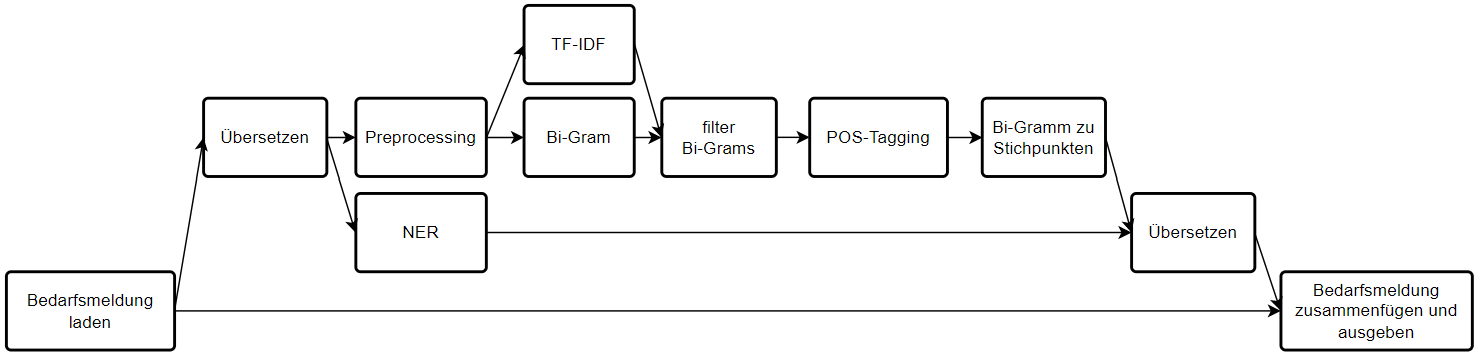
\includegraphics[width=\linewidth]{Abbildungen/flowchart.png}
	\caption{Flussdiagramm der Pipeline.}
	\label{fig:flowchart}
\end{figure}\mbox{} \\
Die Abbildung \ref{fig:flowchart} zeigt das UML-Aktivitätsdiagramm der Python Pipeline zur Strukturierung von \emph{Bedarfsmeldungen}. Im ersten Schritt \emph{unstrukturierte Bedarfsmeldung strukturieren} im Ablauf der Pipeline wird eine \emph{Bedarfsmeldung} ausgewählt und in die festgelegte \emph{Bedarfsmeldungsstruktur} aus Kapitel \ref{sec:strukturierungbedarfsmeldung} umgebaut. Die Felder \emph{Einsatzbeginn} und \emph{Einsatzende} werden zu einem Feld \emph{Einsatz} zusammengefügt. Neben den Feldern \emph{Aufgaben} und \emph{Skills} bleiben alle weiteren Felder bis zum letzten Punkt Ausgabe unverändert. Die Felder \emph{Aufgaben} und \emph{Skills} werden jeweils in die Schleife weitergeleitet, wo sie auf Stichpunkte reduziert werden. Der Prozess zur Reduktion durchläuft mehrere Schritte. Zu Beginn werden die Volltexte aus den Feldern im Punkt \emph{ins Englische übersetzen} übersetzt. Anschließend erfolgt im Schritt \emph{Datums-Daten und Zeiten mit NER extrahieren} zum einen die Extrahierung der zeitbezogenen Daten. Darauffolgend wird der Volltext im Punkt \emph{Preprocessing} für die weitere Nutzung vorverarbeitet. Der Grund warum die Extraktion mit \emph{NER} nicht nach der Vorverarbeitung durchgeführt werden kann ist, da im Vorverarbeitungsschritt alle Nummern und somit auch alle zeitbezogenen Daten entfernt werden. Die Resultate des \emph{NER} werden zum Ende hin zurück ins deutsche übersetzt und der fertigen Stichpunktliste beigefügt. Zur Erstellung der Stichpunktliste werden relevante Schlüsselwörter durch die \emph{TF-IDF}-Methode ermittelt. Anschließend wird der vorverarbeitete Text zu \emph{Bi-Grammen} umgeformt. Beim Punkt \emph{Bi-Gramme auf Schlüsselwörter filtern} werden alle \emph{Bi-Gramme} entfernt, die kein Schlüsselwort aus der \emph{TF-IDF}-Methode enthalten. Somit erhält der Schritt \emph{untypische Wortartenkombinationen mit POS-Tagging entfernen} eine reduzierte Liste mit \emph{Bi-Grammen}, bei dem mindestens eines der beiden \emph{Bi-Gramm}-Wörter ein Schlüsselwort Wort darstellt. Jedes Wort der \emph{Bi-Gramm}-Liste durchläuft eine weitere Filterung. Im Englischen existieren Wortarten, die typischerweise nicht nebeneinander stehen. Durch Entfernung dieser \emph{Bi-Gramme} durch POS-Tagging-Kombinationen erfolgt eine weitere Trennung der Wortketten in der \emph{Bi-Gramm}-Liste. Wörter die nicht zusammengehören, verlieren dadurch die Verbindung zueinander. Im darauf folgenden Schritt \emph{Bi-Gramm zu Stichpunkten überführen} werden die \emph{Bi-Gramme} jeweils zu einem String zusammengefügt, bei dem im darauf Folgendem \emph{Bi-Gramm} ebenfalls ein relevantes Wort enthalten sind. Dadurch formt sich eine Liste mit Stichpunkten bestehend aus eins bis x vielen Wörtern, die Bezug zueinander haben. Im Schritt \emph{ins Deutsche übersetzen} wird die Liste mit Stichpunkten zurück ins übersetzt. Dieser Ablauf wird für die beiden Felder \emph{Aufgaben} und \emph{Skills} durchlaufen, da diese Volltextfelder darstellen.
\section{Implementationsdetails}
Dieses Kapitel beschreibt den technischen Entwicklungsprozess zur Umsetzung der Anforderungen des Systems. Die Implementierung fokussiert sich auf die Umsetzungen von Technologien und Funktionsweisen verschiedener Anforderungen. Zudem wird die Struktur des Projektes aufgezeigt.
\subsection{Pipeline}
Die Pipeline wurde in der Programmiersprache Python umgesetzt. Python hat sich zu einer der populärsten interpretierten Programmiersprachen entwickelt \cite{mckinney2012python}. Die Programmiersprache eignet sich insbesondere für die Erstellung kleiner Programme und Skripte, die zur Automatisierung von Aufgaben eingesetzt werden können \cite{mckinney2012python}. Python hat eine große und aktive Community für wissenschaftliche Berechnungen und Datenanalysen hervorgebracht und hat sich in den letzten Jahren zu einer der wichtigsten Sprachen für Data Science, maschinelles Lernen und allgemeine Softwareentwicklung in Wissenschaft und Industrie entwickelt \cite{mckinney2012python}. Python unterstützt Modularität, wodurch ein Teil der Anforderungen somit abgedeckt werden kann. Die Implementierungen der einzelnen Verfahren aus den Anforderungen werden nicht manuell, sondern auf Basis von bereits existierende Bibliotheken umgesetzt.
\subsection{Projektstruktur}
\label{sec:projektstruktur}
Das Projekt wird in einem git Repository gespeichert und versioniert. Die Projektstruktur ist ohne zusätzliche Konfigurationsdateien wie folgt aufgebaut:
\dirtree{%
	.1 .git/.
	.2 modules/.
	.3 ner.py.
	.3 nGram.py.
	.3 posTagging.py.
	.3 preprocessing.py.
	.3 readRequirements.py.
	.3 textRankingAlgorithm.py.
	.3 tfIdf.py.
	.3 transformRequirements.py.
	.3 translate.py.
	.2 requirements/.
	.3 jiraTickets.json.
	.3 preprocessedRequirements.json.
	.3 ....
	.2 app.py.
	.2 ....
}
Die einzelnen Module aus dem Flussdiagramm in Kapitel \ref{fig:flowchart} sind im Verzeichnis \url{modules/} in separaten \url{.py} Dateien gelagert. Die \emph{Bedarfsmeldungen} werden im \url{requirements/}-Verzeichnis gespeichert. Alle relevanten \emph{Bedarfsmeldungen} sind in der \url{jiraTickets.json}-Datei in einer Liste gespeichert. Die Datei \url{app.py} ist der Kern der Pipeline. Diese importiert alle Module und implementiert die Struktur der Pipeline. Das Projekt kann über den Befehl \lstinline{> py app.py} ausgeführt werden.
\subsection{Modulimplementationen}
Nachfolgend werden Implementationsdetails zu den einzelnen Modulen gegeben. Dabei werden verwendete Bibliotheken und Code-Details näher erläutert.
\paragraph{Strukturierung von Bedarfsmeldungen}\mbox{}\\
Die \emph{Bedarfsmeldungen} wurden über die Jira-Schnittstelle extrahiert und im Verzeichnis \url{requirements/jiraTickets.json} gespeichert. Zur Eingrenzung der Datenmenge wurde ein Filter angewendet, der nur die \emph{offenen} und \emph{eskalierten} \emph{Bedarfsmeldungen} zurückgibt. Diese sind die relevanten und noch aktuellen \emph{Bedarfsmeldungen}. Zudem wurden alle unrelevanten Felder mit einem weiteren Filter herausgenommen. Die Daten aus der Jira-API bestehen namentlich aus \emph{customfields} mit einer angehangenden ID. Der Softwareprototyp lädt in dem Modul \emph{readRequirements.py} die unstrukturierten Fields und formt diese in dem Modul \emph{transformRequirements.py} in \emph{Bedarfsmeldungs}-Objekte um.
\begin{center}
	\begin{tabularx}{1\textwidth} { 
			| >{\raggedright\arraybackslash}X 
			| >{\raggedright\arraybackslash}X
			| >{\raggedright\arraybackslash}X | }
		\hline
		Display-Felder & Jira-API-Felder & Objekt-Felder \\
		\hline
		\hline
		Überschrift & summary & header\\
		\hline
		Rolle & customfield\_15321 & role\\
		\hline
		Aufgaben & customfield\_10288 & tasks\\
		\hline
		Skills & customfield\_10296 & skills\\
		\hline
		Skill-Level & customfield\_15322 & skillLevel\\
		\hline
		Kunde & customfield\_10279 & customer\\
		\hline
		Einsatzort & customfield\_10297 & location\\
		\hline
		Beginn & customfield\_10293 & timePeriod\\
		\hline
		Ende & customfield\_10294 & timePeriod\\
		\hline
		Tagessatz & customfield\_10298 & dailyRate\\
		\hline
	\end{tabularx}\\
	\captionof{table}{Übersicht der Datenfelder}
	\label{tab:jiradaten}
\end{center}
In der Tabelle \ref{tab:jiradaten} ist in der ersten Spalte eine Übersicht der Datenfelder, wie diese in der Abbildung \ref{fig:jiraafter} mit dem Mockup einer standardisierten \emph{Bedarfsmeldung} auftauchen. In der zweiten Spalte sind die dazugehörigen Feldernamen, die in der \url{jiraTickets.json} enthalten sind. Die dritte Spalte spiegelt die jeweiligen Namen innherhalb des  \emph{Bedarfsmeldungs}-Objekts im Prototypen wieder. Das  \emph{Bedarfsmeldungs}-Objekt dient der strukturierten Handhabung der \emph{Bedarfsmeldungs}-Daten innerhalb des Systems.

%Um einen Freitext aus einer einzelnen \emph{Bedarfsmeldung} für die Pipeline zu laden werden Daten mit der Endung \url{.txt} verwendet.
%\begin{lstlisting}[caption={Implementation der Methode read() des Moduls \emph{readRequirements.py}}, label=lst:read]
%	def read(filename):
%		path = os.path.join(PATH, filename)
%		file = open(path, "r", encoding="utf-8")
%		content = file.read()
%		file.close()
%		return content
%\end{lstlisting}
%Im Listing \ref{lst:read} ist die Implementierung der Methode zum laden eines Freitextes dargestellt. Durch ein mitgelieferten Parameter \emph{filename} wird der Name der Datei in Zeile 2 an den Pfad angehängt. Mit der Methode \lstinline{open()}
%aus Zeile 3 kann die Datei geladen werden. Die Methode erhält die Parameter Pfad, \emph{'r'} (read) und das encoding \emph{'utf-8'}. Das encoding ist dabei Entscheidend, damit die unstrukturierten \emph{Bedarfsmeldungen} laden können. Bei der Pflege in Jira wird wenig Wert auf eine einheitliche Struktur. Somit können Zeichen enthalten sein, die beim öffnen nicht erkannt werden und eine Fehlermeldung wird zurückgegeben. Zur Vermeidung dieses Fehlers wird das encoding festgelegt. Nach dem laden durch die Methode \lstinline{read()} wird der Inhalt der \url{.txt} Datei in der Variable \emph{content} gespeichert und zurückgegeben.
\paragraph{Übersetzung}\mbox{}\\
Das Modul \emph{translate.py} ist dazu da, um die \emph{Bedarfsmeldungen} zu übersetzen. Für die Übersetzung wurde die Python Bibliothek \emph{deep-translator} verwendet. Diese bietet Implementationen unterschiedlicher Übersetzungs-APIs von diversen Anbietern. Der Vorteil ist dabei die vereinfachte Möglichkeit Anbieter bei Bedarf zu wechseln.
%\begin{lstlisting}[caption={Implementation des Moduls \emph{translate.py}}, label=lst:translate]
%	from deep_translator import GoogleTranslator
%	
%	def translate(text):
%		translated = GoogleTranslator(source='auto', target='en').translate(text)
%		return translated
%\end{lstlisting}
%Das Listing \ref{lst:translate} zeigt die Implementation des Moduls. 
Es wurde sich für den Google Translator entschieden, da hierfür kein API-Key benötigt wird. Die Methode erhält einen Text als Parameter. Der Google Translator erhält die Parameter \emph{source} und \emph{target}, beidem \emph{source} angibt in welcher Sprache der Eingabetext ist. Durch Angabe von \emph{'auto'} wird die Sprache ermittelt. Der Grund dafür ist, dass grundsätzlich anderssprachige \emph{Bedarfsmeldung} enthalten sein können. Der Parameter \emph{target} ist die Zielsprache in welche der Input übersetzt werden soll. Die Zielsprache ist hier Englisch (\emph{'en'}).
\paragraph{NER}\mbox{}\\
Um die Methode \emph{NER} zu Implementieren wurde die Bibliothek \emph{spaCy} und das Modell \emph{en\_core\_web\_sm} verwendet. 
%\begin{lstlisting}[caption={Implementation des Moduls \emph{ner.py}}, label=lst:ner]
%	import spacy
%	nlp = spacy.load("en_core_web_sm")
%	ner_categories = ["ORG","FAC","GPE","PRODUCT", "EVENT", "LANGUAGE", "DATE", "QUANTITY"]
%	def useNER(requirement):
%		tokenized = nlp(requirement)
%		entities = []
%		for ent in tokenized.ents:
%			if ent.label_ in ner_categories:
%				entities.append((ent.text, ent.label_))
%	return entities
%\end{lstlisting}
Die zu extrahierende Kategorie ist Datum (DATE). Innerhalb der Methode \lstinline{useNER()} wird der Volltext als Parameter übergeben und zu Tokens umgeformt. Anschließend werden alle Tokens durchlaufen und nach ihren Kategorien überprüft. Ist ein Token die definierte Kategorie, wird der Token in eine separate Liste gespeichert und zurückgegeben. Die extrahierten Tokens werden aus dem Volltext entfernt, um am ende keine doppelten Stichpunkte zu erhalten.
\paragraph{Preprocessing}\mbox{}\\
Vor der weiteren Nutzung der Daten innerhalb einer \emph{Bedarfsmeldung}, ist es erforderlich diese von irrelevanten Wörtern, Zeichen und Formatierungen zu befreien.% Zur Entfernung von Satzzeichen wurde die Bibliothek \emph{string} verwendet.
%\begin{lstlisting}[caption={Implementation der Methode removePunctuation() des Moduls \emph{preprocessing.py}}, label=lst:punctuation]
%	import string
%	def removePunctuation(text):
%		content=""
%		for i in text: 
%			if i not in string.punctuation:
%				content+=i    
%		return content
%\end{lstlisting}
%Im Listing \ref{lst:punctuation} ist die Implementierung dargestellt. Die \emph{Bedarfsmeldung} wird in Zeile 2 als Parameter übergeben. In Zeile 4 erfolgt ein Durchlauf jedes Zeichens innerhalb der \emph{Bedarfsmeldung}. Falls innerhalb der Schleife das Aktuelle Zeichen kein Satzzeichen enthält wird dieses in die Variable \emph{content} zwischengespeichert. Nach Abschluss der Schleife wird die Variable zurückgegeben. 
Zur Eliminierung wiederaufgetretener Wörter, die keine Relevanz für den Informationsgehalt aufweisen, wurde die Bibliothek \emph{nltk} verwendet. Diese beinhaltet eine Liste an sogenannten \emph{stopwords}.
%\begin{lstlisting}[caption={Implementation der Methode removeStopwords() des Moduls \emph{preprocessing.py}}, label=lst:stopwords]
%	from nltk.corpus import stopwords
%	def removeStopwords(text):
%		words=[word for word in text.split(" ") if word not in set(stopwords.words('english'))]
%		return " ".join(str(word) for word in words)
%\end{lstlisting}
%Im Listing \ref{lst:stopwords} ist die Implementierung zur Entfernung von \emph{stopwords} dargestellt. In Zeile 3 
Es werden alle mit einem Leerzeichen getrennten Wörter aus der übergebenen \emph{Bedarfsmeldung} in einer Liste aufgeteilt. Dabei wird jeder Listeneintrag mit der \emph{stopword}-Liste von \emph{nltk} verglichen. Stimmt das Wort nicht mit einem Eintrag der \emph{stopwords} überein, wird diese in die Liste \emph{words} hinzugefügt. Zum Schluss werden die Wörter wieder zu einem String zusammengetragen und zurückgegeben. \\

Um weitere Formatierungen und ungewünschte Zeichen zu entfernen wird die Bibliothek \emph{re} verwendet. Diese kann Regular Expression-Patterns anwenden und Bereiche, die zum Pattern passen entfernen.
%\begin{lstlisting}[caption={Implementation der Methode removeTags() und removeSpecialCharactersAndDigits() des Moduls \emph{preprocessing.py}}, label=lst:re]
%	import re
%	def removeTags(text):
%		return re.sub("</?.*?>"," <> ",text)
%	
%	def removeSpecialCharactersAndDigits(text):
%		return re.sub("(\\d|\\W)+"," ",text)
%\end{lstlisting}
%Im Listing \ref{lst:re} sind Implementationsdetails zur Entfernung von Tags und ungewollte Zeichen dargestellt. 
Die Methode \lstinline{removeTags()} erhält die Expression \lstinline{</?.*?>}. Dabei werden \lstinline{<Tags>} ermittelt und mit der Methode \lstinline{sub()} entfernt. Zur Entfernung von Ziffern und Nicht-Alphanummerischen Zeichen wird die Expression \lstinline{(\\d|\\W)+} angewendet. Als Ergebnis des Preprocessing wird ein gesäuberter String ohne Zeichen und Tags zurückgegeben. Zum schluss werden alle Wörter in Kleinbuchstaben umgewandelt. Der Grund dafür ist, dass somit die Vergleichbarkeit der Wörter gefördert wird. Es könnte sonst vorkommen, dass Beispielsweise beim Schlüsselwörterabgleich zwei Wörter nicht als identisch identifiziert werden, da sie einmal mit großem und eimal mit kleinem Anfangsbuchstaben geschrieben wurde.
\paragraph{TF-IDF}\mbox{}\\
Vorbereitend für die \emph{TF-IDF}-Methode wurden die \emph{Skills} und \emph{Aufgaben} aus allen \emph{Bedarfsmeldungen} ins Englische übersetzt, Preprocessed und in einem String zusammengefasst. Der Grund dafür ist, dass für die \emph{TF-IDF}-Methode ein Textkorpus benötigt wird, woraus die Schlüsselwörter durch \emph{Term Frequency} ermittelt werden. Damit dieser Prozess nur einmal erfolgen muss, wurden die Ergebnisse in die \url{requirements/preprocessedRequirements.json} gespeichert. Für die Implementierung des \emph{TF-IDF} wurden die Bibliotheken \emph{sklearn} und \emph{numpy} verwendet. Der Textkorpus wird dem \emph{TfidfVectorizer} von \emph{sklearn} beigefügt und die \emph{TF-IDF}-Werte werden berechnet. Anschließend werden alle durchschnittlichen \emph{TF-IDF}-Werte für jedes Wort im gesamten Textkorpus berechnet. Daraus wird eine Liste mit Wörtern und ihren durchschnittlichen \emph{TF-IDF}-Werten erstellt und in absteigender Reihenfolge sortiert. Durch ein vordefinierten Score Threshold können darunterliegende Schlüsselwörter entfernt werden. Dies ist wichtig, damit Wörter mit niedrigem Scoring und diese Beispielsweise nur einmal im Textkorpus auftauchen nicht als Schlüsselwörter erfasst werden. Als Ergebnis wird eine Liste mit Schlüsselwörtern zurückgegeben.

%\begin{lstlisting}[caption={Implementation des Moduls \emph{tfIdf.py}}, label=lst:postagging]
%import modules.readRequirements as readRequirements
%from sklearn.feature_extraction.text import TfidfVectorizer
%import numpy as np
%def useTfIdf(text):
%	object = readRequirements.loadJson("preprocessedRequirements.json")
%	documents = [object['tasks'], object['skills']]
%	vectorizer = TfidfVectorizer()
%	tfidf_matrix = vectorizer.fit_transform(documents)
%	feature_names = vectorizer.get_feature_names_out()
%	avg_tfidf_scores = np.mean(tfidf_matrix.toarray(), axis=0)
%	tfidf_scores = list(zip(feature_names, avg_tfidf_scores))
%	sorted_tfidf_scores = sorted(tfidf_scores, key=lambda x: x[1], reverse=True)
%	score_threshold = 0.1
%	filtered_keywords = [word for word, score in sorted_tfidf_scores if score > score_threshold]
%	return filtered_keywords
%\end{lstlisting}

%\paragraph{TextRank}\mbox{}\\
%Für die Implementation von \emph{TextRank} wurde die Bibliothek \emph{spaCy} und \emph{pytextrank} verwendet. Dieses bietet die NLP-Pipeline \emph{en\_core\_web\_sm}, das mit Internettext vortrainiert wurde und Vokabeln, Syntax und Entitäten enthält.
%\begin{lstlisting}[caption={Implementation des Moduls \emph{textRankingAlgorithm.py}}, label=lst:textrank]
%	import spacy
%	import pytextrank
%	def useTextRank(requirement):
%		nlp = spacy.load("en_core_web_sm")
%		nlp.add_pipe("textrank")
%		tokenized = nlp(requirement)
%		for phrase in tokenized._.phrases:
%			print(phrase.text)
%			print(phrase.rank, phrase.count)
%			print(phrase.chunks)
%\end{lstlisting}
%Das Listing \ref{textrank} zeigt die Implementierung des \emph{textRankingAlgorithm.py} Moduls. In Zeile 3 wird die \emph{Bedarfsmeldung} als Parameter übergeben. Die Pipeline \emph{en\_core\_web\_sm} wird in Zeile 4 geladen und in Zeile 5 werden die \emph{TextRank} Elemente der Pipeline hinzugefügt. Anschließend wird in Zeile 6 die \emph{Bedarfsmeldung} der Pipeline eingefügt und in Tokens umgewandelt.\\
%\todo{muss noch fertiggestellt werden}\\
\paragraph{N-Gramm}\mbox{}\\
Damit wie in Kapitel \ref{sec:anforderungsanalyse} Wortketten gebildet werden können ist es notwendig \emph{bi-Gramme} zu verwenden, da somit immer zwei nebeneinanderstehenden Wörter betrachtet werden können. Bei einem höheren n der \emph{n-Gramme} würde somit das Prinzip einer Wortkette, wie sie im System benötigt wird nicht funktionieren. Die Methode der \emph{n-Gramme} wurde mit der Bibliothek \emph{nltk} implementiert.
%\begin{lstlisting}[caption={Implementation des Moduls \emph{nGram.py}}, label=lst:ngram]
%	from nltk import ngrams
%	n = 2
%	def useNGram(text):
%		nGramList = []
%		nGrams = ngrams(text.split(), n)
%		for grams in nGrams:
%			nGramList.append(grams)
%		return nGramList
%\end{lstlisting}
%Das Listing \ref{lst:ngram} zeigt die Implementation des Moduls \emph{nGram.py}. 
Eine Variable \emph{n} ist definiert, die die Größe eines \emph{n-Gramms} widerspiegelt. Da in der Pipeline \emph{Bi-Gramme} benötigt werden, liegt der Wert von n auf 2. Mit der Methode \lstinline{ngrams()}
können die \emph{n-Gramme} generiert werden. Diese erhalten einen \emph{String} und die Variable \emph{n} als Parameter. Der zu überführende Text wird als Parameter übergeben und durch die Methode \lstinline{split()}
in einer List auf die einzelnen Wörter umgeformt. Die einzelnen Tupel mit den \emph{Bi-Grammen} werden am Ende zurückgegeben.
\paragraph{Entfernung von Bi-Grammen ohne Schlüsselwörter}\mbox{}\\
Zur Entfernung von Bi-Gramm-Tupel, die keine Schlüsselwörter enthalten wurde die Methode \lstinline{containsKeywords()} erstellt.
\begin{lstlisting}[caption={Implementation der Filterung für Schlüsselwörter in einer Bi-Gramm Liste}, label=lst:bigram]
	def containsKeywords(biGramList, keywordsList):
		filteredBiGram = []
		for tupel in biGramList:
			if any(word in tupel for word in keywordsList):
				filteredBiGram.append(tupel)
		return filteredBiGram
\end{lstlisting}
Das Listing \ref{lst:bigram} implementiert diese Methode. Als Parameter wird die \emph{Bi-Gramm}-Liste und die Schlüsselwörterliste übergeben. In Zeile 3 ist zu sehen, dass jeder Tupel traversiert wird. Dabei wird in Zeile 4 jedes Wort im Tupel mit der Schlüsselwörterliste verglichen. Wenn das aktuelle Wort in der Liste enthalten ist, so wird dieser Tupel in eine neue Liste aufgenommen. Diese wird am Ende zurückgegeben, wodurch eine gefilterte Liste mit ausschließlich enthaltenen Schlüsselwörtern vorhanden ist.
\paragraph{POS-Tagging}\label{postagging} \mbox{}\\
In der Englischen Sprache existieren verschiedene Wortgruppenkombinationen, die zusammen ungewöhnlich klingen und dadurch beim sprechen und schreiben nicht oder nur selten verwendet werden. Wenn diese Kombinationen in den \emph{Bi-Grammen} identifiziert und entfernt werden, können somit Verbindungsketten unterbrochen werden. Dadurch stehen Wörter und spätere Stichpunkte nicht nebeneinander, die sprachlich im betrachteten Kontext wenig Sinn machen. \emph{Bedarfsmeldungen} wurden im professionell seriösen Kontext angefertigt, wodurch einige nebeneinanderstehenden Wörter im Englischen nicht häufig zusammen auftauchen.
\begin{center}
	\begin{tabularx}{1\textwidth} { 
			| >{\raggedright\arraybackslash}X 
			| >{\raggedright\arraybackslash}X
			| >{\raggedright\arraybackslash}X | }
		\hline
		Wortarten & POS-Tagging Abkürzungen & Beispiel \\
		\hline
		\hline
		Nomen + Adjektiv & NN JJ & "time beautiful"\\
		\hline
		Verb + Adjektiv & VB JJ & "think beautiful"\\
		\hline
		Verb + Pronomen & VB PRP & "think him"\\
		\hline
		Verb + Verb & VB VB & "think understand"\\
		\hline
		Adjektiv + Adjektiv & JJ JJ & beautiful strange\\
		\hline
		Adjektiv + Verb & JJ VB & beautiful think\\
		\hline
		Adjektiv + Adverb & JJ RB & "beautiful fast"\\
		\hline
		Adverb + Adjektiv & RB JJ & "fast beautiful"\\
		\hline
	\end{tabularx}\\
	\captionof{table}{Untypische Wortartenkombinationen in der englischen Sprache.}
	\label{tab:wortkombinationen}
\end{center}
In der Tabelle \ref{tab:wortkombinationen} sind einige Beispiele für solche ungewöhnlichen Zusammensetzungen. In Spalte eins sind die jeweiligen Wortarten beschrieben. Die zweite Spalte zeigt die dazugehörigen Tags, wie diese mit \emph{POS-Tagging} ermittelt werden. Die dritte Spalte zeigt jeweils ein Beispiel dieser Wortkombinationen. Die Identifikation erfolgte durch Betrachtung der Grundregeln der Englischen Grammatik aus der Arbeit \citetitle{ogden1930basic}\cite{ogden1930basic} und den Syntaxregeln aus der Arbeit \citetitle{tayal2014syntax}\cite{tayal2014syntax}. Diese Regeln beinhalten Kombinationen aus Wortarten, die zusammen Erlaubt sind. Dadurch konnten Kombinationen ausgeschlossen werden. Schließlich wurden durch trial and error weitere Kombinationen identifiziert, die schließlich in die Tabelle aufgenommen wurden. Es kann nicht ausgeschlossen werden, dass weitere Kombinationen und Sonderfälle existieren. Dies stellt ein Optimierungspotenzial außerhalb dieser Ausarbeitung dar. Somit werden nur die Kombinationen aus der Tabelle \ref{tab:wortkombinationen} im System beachtet. Dennoch ist dieses so konzipiert, dass weitere Kombinationen in das System hinzugefügt werden können.\\

Zur Implementierung der Methode \emph{POS-Tagging} wurde die Bibliothek \emph{nltk} verwendet. Die \emph{Tags} werden mit dem vortrainierten Modell \emph{averaged\_perceptron\_tagger} ermittelt.
%\begin{lstlisting}[caption={Implementation des Moduls \emph{posTagging.py}}, label=lst:postagging]
%	import nltk
%	nltk.download('averaged_perceptron_tagger')
%	def usePosTagging(text):
%		tokens = nltk.word_tokenize(text)
%		pos_tags = nltk.pos_tag(tokens)
%		return pos_tags
%\end{lstlisting}
%Im Listing \ref{lst:postagging} sind Details zur Implementierung dargestellt. 
Als Parameter wird ein String übergeben, der zwei Wörter aus den \emph{Bi-Grammen} enthält. Dieser String wird in Tokens umgewandelt. Diese werden in die Methode \lstinline{pos_tag()}
übergeben und eine Liste mit Tupeln wird zurückgegeben, bei dem das Wort und das dazugehörige \emph{Tag} enthalten ist.
\paragraph{Entfernung von Bi-Grammen mit ungewöhnlichen Wortartenkombinationen}\mbox{}\\
Die \emph{Bi-Gramm}-Liste muss im nächsten Schritt weiter reduziert werden. Hierbei werden alle \emph{POS-Tagging}-Kombinationen aus der Tabelle \ref{tab:wortkombinationen} mit den Tupeln aus der \emph{Bi-Gramm}-Liste verglichen werden.
\begin{lstlisting}[caption={Implementation der Filterung von Wortartenkombinationen}, label=lst:wortarten]
	combinationsToRemove = ["NN JJ", "VB JJ", "VB PRP", "VB VB", "JJ JJ", "JJ VB", "JJ RB", "RB JJ"]
	def removeWordCombination(biGramList):
		filteredList = []
		for left, right in biGramList:
			biGramString = f"{left} {right}"
			biGramStringsWithTags = usePosTagging(biGramString)
			tagString = ' '.join(tag for _, tag in biGramStringsWithTags)
			if tagString not in combinationsToRemove:
				filteredList.append((left, right))
		return filteredList
\end{lstlisting}
Das Listing \ref{lst:wortarten} implementiert diesen Schritt. Dazu werden in Zeile 1 alle Kombinationen als String in eine Liste zwischengespeichert. Als Parameter wird die zu filternde \emph{Bi-Gramm}-Liste übergeben. Diese wird in Zeile 4 traversiert und die Tupel mit den beiden Wörtern aus den \emph{Bi-Grammen} wird in Zeile 5 als String zusammengefügt. Dieser String wird in die \emph{POS-Tagging}-Methode übergeben und als Rückgabewert erhält das System eine Liste mit zwei Tupeln. Diese Tupel beinhalten jeweils eines der Wörter und das dazugehörige Tag aus dem \emph{POS-Tagging}. Die beiden Tags werden in Zeile 7 zusammengefügt, sodass ein String entsteht, wie es in der \emph{combinationsToRemove}-Liste in Zeile 1 ist. In Zeile 8 wird überprüft ob die Kombination aus Tags einer aus der Liste in Zeile 1 entspricht. Ist dies nicht der Fall, wird der Tupel in eine neue Liste eingefügt, die am Ende als Ausgabe zurückgegeben wird.
\paragraph{Überführung von Bi-Grammen in Stichpunkte}\label{par:stichpunkte}\mbox{}\\
Da der Volltext aus den Bedarfsmeldungen nicht einzelne Wörter, sondern inhaltlich aufeinander bezogene Stichpunkte entstehen sollen, werden die um die Schlüsselwörter herumliegenden Wörter aneinander gefügt. Dazu werden diejenigen \emph{Bi-Gramme} zu einem Satz zusammengefügt, die im ersten Tupel auf der rechten Seite und im zweiten Tupel auf der linken Seite das gleiche Wort enthalten. Hinzu kommt eine Überprüfung ob das darauffolgende linke Wort ein Schlüsselwort ist. Somit werden nur die Wörter zu Sätzen verkettet, die aus Schlüsselwörtern bestehen. In dem Fall, bei dem im darauf folgenden Tupel kein Schlüsselwort auf der linken sondern nur auf der rechten besteht, entsteht ein neuer Stichpunkt. Als Beispiel können folgende \emph{Bi-Gramme} betrachtet werden: (\grqq expertise\grqq, \grqq aws\grqq) (\grqq aws\grqq, \grqq technologie\grqq) (\grqq technologie\grqq, \grqq pflicht\grqq) (\grqq pflicht\grqq, \grqq englisch\grqq) (\grqq englisch\grqq, \grqq skills\grqq). Als Schlüsselwörter wurden die Wörter \grqq aws\grqq, \grqq pflicht\grqq, \grqq englisch\grqq ermittelt. Die Idee ist es, die zusammengehörigen \emph{Bi-Gramme} an diesen Schlüsselwörtern zusammenzufügen. Daraus werden die Stichpunkte \grqq expertise aws technologie\grqq und \grqq technologie pflicht englisch skills\grqq.
\begin{lstlisting}[caption={Umformung der Bi-Gramm Liste in Stichpunkte}, label=lst:stichpunkte]
	def combineWords(filteredBiGram, keywords):
		combinedWords = []
		i = 0
		while i < len(filteredBiGram):
			keyPhrase = recursivCombine(filteredBiGram, i, "", keywords, "")
			combinedWords.append(keyPhrase)
			wordsCount = len(keyPhrase.split(" "))
			wordsCount = max(1, wordsCount - 1)
			i += wordsCount
			if(i > len(filteredBiGram)):
				break
		return combinedWords
	
	def recursivCombine(filteredBiGram, index, currentString, keywords, lastRightItem):
		left, right = filteredBiGram[index]
		if not currentString:
			currentString = left
		else:
			currentString += " " + left
		if lastRightItem in {left, ""}:
			if right in keywords and index + 1 < len(filteredBiGram):
				currentString = recursivCombine(filteredBiGram, index + 1, currentString, keywords, right)
			else:
				currentString += " " + right
		return currentString
\end{lstlisting}
Die Implementierung zu dieser Idee ist im Listing \ref{lst:stichpunkte} dargestellt. Die Methode \lstinline{combineWords} in Zeile 1 erhält die \emph{Bi-Gramm}-Liste und die Schlüsselwörterliste als Parameter. Die \emph{Bi-Gramm}-Liste wird traversiert und ein string aus zusammengehörigen Wörtern wird rekursiv in Zeile 5 mit der Methode \lstinline{recursivCombine} erstellt. Dazu wird in jedem rekursiven Schritt überprüft, ob das darauf folgende rechte wort ein Schlüsselwort und das gleiche wie das linke Wort im aktuellen Tupel entspricht. Ist dies der Fall werden die \emph{bi-Gramm} an der Stelle zusammengefügt. Dies wiederholt sich bis dieser Fall nicht mehr eintritt. Dadurch ist die Rekursion vorbei und ist wird in Zeile 7 bis 11 geprüft wie viele Wörter in einem String gelandet sind. Das ist wichtig um herauszufinden an welcher Stelle in der \emph{bi-Gramm}-Liste weiter gearbeitet werden muss. Sind alle \emph{bi-Gramme} zusammengesetzt worden, wird eine Liste mit allen zusammengesetzten Wörtern zurückgegeben.
\section{Erklärung des Systems anhand eines Beispiels}
Nachfolgend wird zum besseren Verständnis die Schritte zur Verarbeitung eines Volltextes anhand eines konkreten Beispiels dargestellt.\\
\begin{enumerate}
	\item Zu Beginn haben wir folgenden Volltext:\\ \textbf{Für verschiedene IT-Projekte (mit internen und externen Kunden) benötigen wir Unterstützung von einem Projektleiter, mit Erfahrungen in der Planung, Koordination und Durchführung von IT-Migrations- und Implementierungsprojekten im Umfeld von Rechenzentrumsservices. Mindestens 2 Jahre Erfahrung sind erwünscht.}
	\item Dieser Text wird übersetzt:\\ \textbf{For various IT projects (with internal and external customers) we need support from a project manager with experience in planning, coordinating and executing IT migration and implementation projects in the area of data center services. At least 2 years of experience is desired.}
	\item Nun werden aus dem Text Datums- und Zeitangaben extrahiert und aus dem Volltext entnommen:\\ \textbf{At least 2 years \grqq Der neue Text beinhaltet: \grqq For various IT projects (with internal and external customers) we need support from a project manager with experience in planning, coordinating and executing IT migration and implementation projects in the area of data center services. of experience is desired.}
	\item Als nächstes wird der Text Vorverarbeitet:\\ \textbf{for various it projects internal external customers need support project manager experience planning coordinating executing it migration implementation projects area data center services experience desired}
	\item Die Schlüsselwörter bestehen unter anderem aus:\\ \textbf{planning, coordinating, migration, implementation, data, center, services, ...}
	\item Aus dem Volltext werden diese \emph{bi-Gramme} erstellt:\\ \textbf{('for', 'various'), ('various', 'it'), ('it', 'projects'), ('projects', 'internal'), ('internal', 'external'), ('external', 'customers'), ('customers', 'need'), ('need', 'support'), ('support', 'project'), ('project', 'manager'), ('manager', 'experience'), ('experience', 'planning'), ('planning', 'coordinating'),
	('coordinating', 'executing'), ('executing', 'it'), ('it', 'migration'), ('migration', 'implementation'), ('implementation', 'projects'), ('projects', 'area'), ('area', 'data'), ('data', 'center'), ('center', 'services'), ('services', 'experience'), ('experience', 'desired')}
	\item Anschließend werden alle \emph{bi-Gramme} ohne Schlüsselwort entfernt:\\ \textbf{('support', 'project'), ('project', 'manager'), ('manager', 'experience'), ('experience', 'planning'), ('planning', 'coordinating'), ('coordinating', 'executing'), ('it', 'migration'), ('migration', 'implementation'), ('implementation', 'projects'), ('area', 'data'), ('data', 'center'), ('center', 'services'), ('services', 'experience'), ('experience', 'desired')}
	\item Der nächste Schritt beinhaltet die Entfernung von ungewöhnlichen \emph{POS-Tagging}-Kombinationen. In diesem Beispiel sind alle Kombinationen zulässig, weswegen die \emph{bi-Gramm}-Liste unverändert bleibt.
	\item Nun werden die \emph{bi-Gramme} nach dem Verfahren aus Kapitel \ref{par:stichpunkte} in folgende Stichpunkte zusammengetragen:\\ \textbf{support project manager, manager experience planning coordinating executing, it migration implementation projects, area data Center services experience desired}.\\ \\ Hinzu kommen die Daten aus dem \emph{NER}-Schritt:\\ \textbf{At least 2 years}
	\item Nach der Übersetzung ist das Ergebnis: \textbf{\begin{itemize}\item Unterstützung des Projektleiters \item Manager Erfahrung Planung Koordinierung Durchführung \item Projekte zur Implementierung von IT-Migrationen \item Erfahrung im Bereich Rechenzentrumsdienstleistungen erwünscht \item Mindestens 2 Jahre \end{itemize}}
\end{enumerate}

%\chapter{Umsetzung der Visualisierungsmethoden}
\label{chap:implementation}
-Wie können diese Art und Weisen mit dem „adesso Staffing Advisor“ Lab implementiert werden

\section{World Cloud}

\newpage

\chapter{Evaluation}
\label{chap:auslieferung}
%\section{SSO ADFS}

-Evaluation der Art und Weisen der KI-Test- und Überwachungsmethoden (Wie hilfreich sind die unterschiedlichen Methoden, vielleicht mit einem Bewertungssystem im „adstaff lab“)
Dashboard mit vielen verschiedenen Methoden der Visualisierung. Jede Methode hat einen eigenen Bereich, wo z.B. Sterne vergeben werden können.


\newpage

\chapter{Zusammenfassung und Ausblick}
\label{chap:ergebnisse}

ergebnis der arbeit: diese modelle in der reihenfolge kommen am nähesten an die bedarfsmeldung

\subsection*{Ausblick}
-die keyword extraction auch für die profile nutzen 
-genauer untersuchen wie einzelne ansätze mit anderen nlp vortrainierten datensätzen abschneidet
-in bezug zu recommender systems beschreiben wie damit weiter gemacht werden könnte
\newpage


\hiddenchapter{Eigenständigkeitserklärung}
Hiermit versichere ich, dass ich die vorliegende Arbeit selbständig angefertigt und mich keiner fremden Hilfe bedient sowie keine anderen als die angegebenen Quellen und Hilfsmittel benutzt habe. Alle Stellen, die wörtlich oder sinngemäß veröffentlichten oder nicht veröffentlichten Schriften und anderen Quellen entnommen sind, habe ich als solche kenntlich gemacht.\\

Diese Arbeit hat in gleicher oder ähnlicher Form noch keiner Prüfungsbehörde vorgelegen.\\
\section*{Erklärung zu eingesetzten Hilfsmitteln}
\begin{enumerate}
	\item Korrekturservice der Fachhochschule bzw. des Fachbereichs genutzt:
	\begin{todolist}
		\item Ja
		\item[\wontfix] Nein
	\end{todolist}
	\item Einsatz eines externen (kommerziellen) Korrekturservice:
	\begin{todolist}
		\item Ja
		\item[\wontfix] Nein
	\end{todolist}
	\item Folgende Personen haben die Arbeit zusätzlich Korrektur gelesen:
	\begin{itemize}
		\item Natascha Schröder
	\end{itemize}
	\item Nutzung von Sprachmodellen für die Texterstellung (z.B. ChatGPT), wenn ja, welche und in welchen Abschnitten:
	\begin{todolist}
		\item Ja
		\item[\wontfix] Nein
	\end{todolist}
	\item Sprachübersetzungstools (z.B. Google Übersetzer, DeepL), wenn ja, welche und in welchen Abschnitten:
	\begin{todolist}
		\item[\wontfix] Ja
		\item Nein
	\end{todolist}
	\begin{itemize}
		\item DeepL, Im Kapitel Literaturüberblick für das bessere Verständnis der Literatur und zur unterstützten Anfertigung des englischen Abstracts
	\end{itemize}
	\item Einsatz von Software zur Sprachkorrektur (z.B. Grammarly), wenn ja, welche und in welchen Abschnitten:
	\begin{todolist}
		\item Ja
		\item[\wontfix] Nein
	\end{todolist}
	\item Einsatz anderer Hilfsmittel:
	\begin{itemize}
		\item 
	\end{itemize}
	\item Ich stimme dem möglichen Einsatz von Software zur Plagiatserkennung zu:
	\begin{todolist}
		\item[\wontfix] Ja
		\item Nein
	\end{todolist}
\end{enumerate}

Ich bestätige, dass obige Aussagen vollständig und nach bestem Wissen ausgefüllt wurden.\\

Dortmund, den \today \\ \\ \\
\begin{tabular}{@{}l@{}}\hline
	Ricardo Valente de Matos
\end{tabular}

%\bibliographystyle{IEEEtranS}
%\bibliography{Literatur}
\raggedright
\printbibliography

\end{document}
